%Introducci�n al cap�tulo...

%--------------------------------------------------
\section{Contexto del sistema}

	La cl\'inica m\'edica de homeopat\'ia requiere de un sistema que realice las funciones y lleve el control de las citas por internet, llevar control sobre inventarios en farmacia as\'i como los expedietes m\'edicos, con el fin de garantizar un mejor servicio a los pacientes de dicha cl\'inica.\\
La cl\'inica cuenta con 12 consultorios y una farmacia, para que una consulta sea llevada a cabo, es necesario que exista una cita previa, ya sea para Consulta General o Especialidad, la diferencia entre ambas es en costo. La cl\'inica cuenta con todas las especialidades, en caso de que no haya cupo en alguna o que no se cuente con dicha especialidad, se mandar\'a al paciente una nueva cl\'inica en la que puede ser atendido.\\
Para sacar una cita no es necesario contar con una afilicaci\'on a la cl\'inica, es abierta a todo p\'ublico, y es posible sacar cita en la cl\'inica o en el sitio web, si la cita se solicita en el sitio web, el paciente (que inicialmente ingresara sus datos) podr\'a seleccionar el consultorio, hora y fecha de la cita, y para recoger la cita en la cl\'inica, debera llegar 10 minutos antes y pagarla para que tenga derecho a dicha cita. De la misma manera puede solicitar la cita en la cl\'inica pagando en caja en ese momento. En caso de que en determinado d\'ia se agoten las citas, se podr\'an reprogramar para otra fecha.\\
La cl\'inica cuenta con una caja en servicio en el que se aceptar\'an todos los pagos de farmacia y consultas.\\
Para acudir a la cita es necesario llegar a tiempo, en caso de que la cita no sea pagada o que el paciente no este presente la cita se puede perder si existe otro paciente esperando.


%--------------------------------------------------
\section{Procesos actuales}
Actualmente en la clinica los documentos e informacion del paciente se lleva de manera escrita.\\
La venta de medicamentos se lleva de manera manuel y hay ocaciones en las que se entregan medicamentos de mas o menos.\\
Tanto la farmacia como el pago de consulta, cuenta con un ticket para comprobar el correcto cobro del servicio.\\

% - - - - - - - - - - - - - - - - - - - - - - - - -
\subsection{Participantes}
\begin{itemize}
    \item Doctor
    \item Cajero
    \item Paciente
    \item Recepcionista
    \item Dependiente
\end{itemize}
% - - - - - - - - - - - - - - - - - - - - - - - - -
\subsection{Procesos}

%diagramas y explicaci�n de los procesos: describir las actividades.

%--------------------------------------------------
\section{Problemas identificados}

% - - - - - - - - - - - - - - - - - - - - - - - - -
\subsection{Problema general}

La clinica actual no cuenta con un sistema optimizado para llevar a cabo el registro de las citas medicas, venta de medicamentos, control de historial medico.

% - - - - - - - - - - - - - - - - - - - - - - - - -
\subsection{Descomposici�n del problema}
\begin{itemize}
    \item No es posible determinar si la farmacia tiene o no ciertos medicamentos por no tener un inventario que lo indique.
	\item No hay manera de llevar un control sobre las citas que los pacientes solicitan (Sitio web).
	\item No se lleva un control, ni seguimiento de los expedientes m\'edicos.
	\item No se conoce el funcionamiento interno en la farmacia, por lo que no se sabe con que frecuencia se surten los medicamentos.
\end{itemize}

% - - - - - - - - - - - - - - - - - - - - - - - - -
\subsection{An�lisis de causas}


\begin{figure}[htbp!]
		\centering
			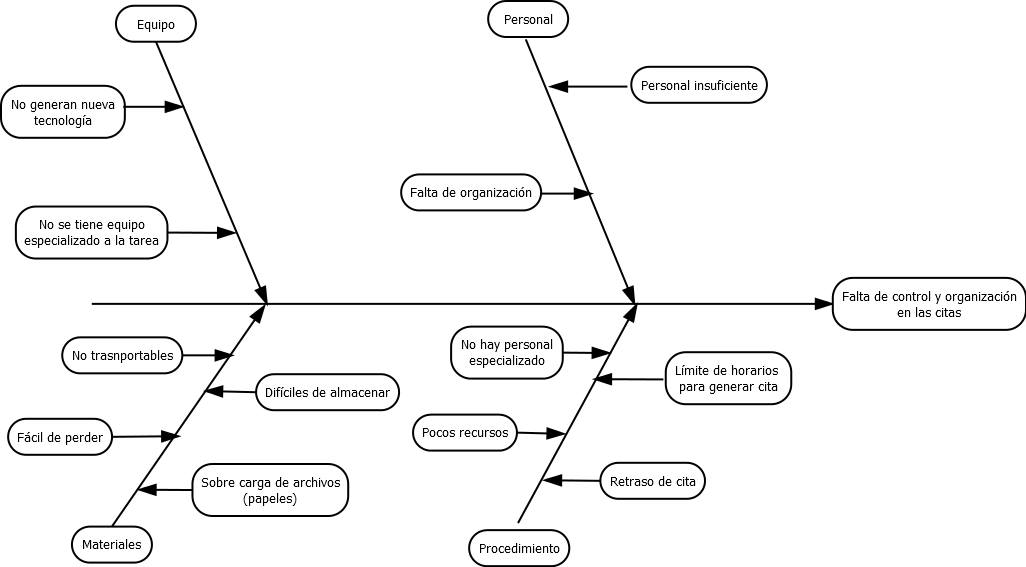
\includegraphics[width=0.8\textwidth]{images/ik}
		\caption{Diagrama de Ishikawa.}
\end{figure}

%--------------------------------------------------
\section{Propuesta de soluci�n}

% - - - - - - - - - - - - - - - - - - - - - - - - -
\subsection{Alternativas de soluci�n}
%Liste las alternativas que encontr� para resolver la problem�tica.